\documentclass[final,t]{beamer}
\usetheme{SJTU}
\usepackage{newtxtext}
\usepackage{amsmath}
\usepackage{bm}
% \usepackage{newtxmath}
\usepackage{booktabs}
\usepackage{tabularx}
\usepackage{minted}
\usepackage{graphicx}
\usepackage{subcaption}
\usepackage[orientation=portrait,size=custom,width=135.46667,height=101.6,scale=1.5]{beamerposter}

% -----------------------------------------
\setbeamerfont{itemize/enumerate subbody}{size=\normalsize}
\title{\Huge Attention Is All You Need}
\author{Ashish Vaswani\inst{1}, Noam Shazeer\inst{1}, Niki Parmar\inst{2}, Jakob Uszkoreit\inst{2}, Llion Jones\inst{2}, Aidan N. Gomez\inst{3}, Łukasz Kaiser\inst{1}, Illia Polosukhin\inst{4}}
\institute[Google, University of Toronto]{
  \inst{1}Google Brain ,
  \inst{2}Google Research,
  \inst{3}University of Toronto,
  \inst{4}Independent Researcher
}
\date[Dec. 2017]{Dec. 2017}
% -----------------------------------------

\begin{document}
\begin{frame}[fragile]{}
  \begin{columns}[t]
    \begin{column}{.3\linewidth}

	\begin{block}{Background}
	\begin{itemize}
	\item RNNs and GRUs have led sequence-based tasks but face parallelization and long-range dependency challenges. CNNs partially address these but fall short. 
	\item The Transformer, revolutionizes this by using attention mechanisms to enhance focus on input sequences and boost parallelization, forgoing traditional sequential processing.
	\end{itemize}
	
	\begin{figure}
		\centering
		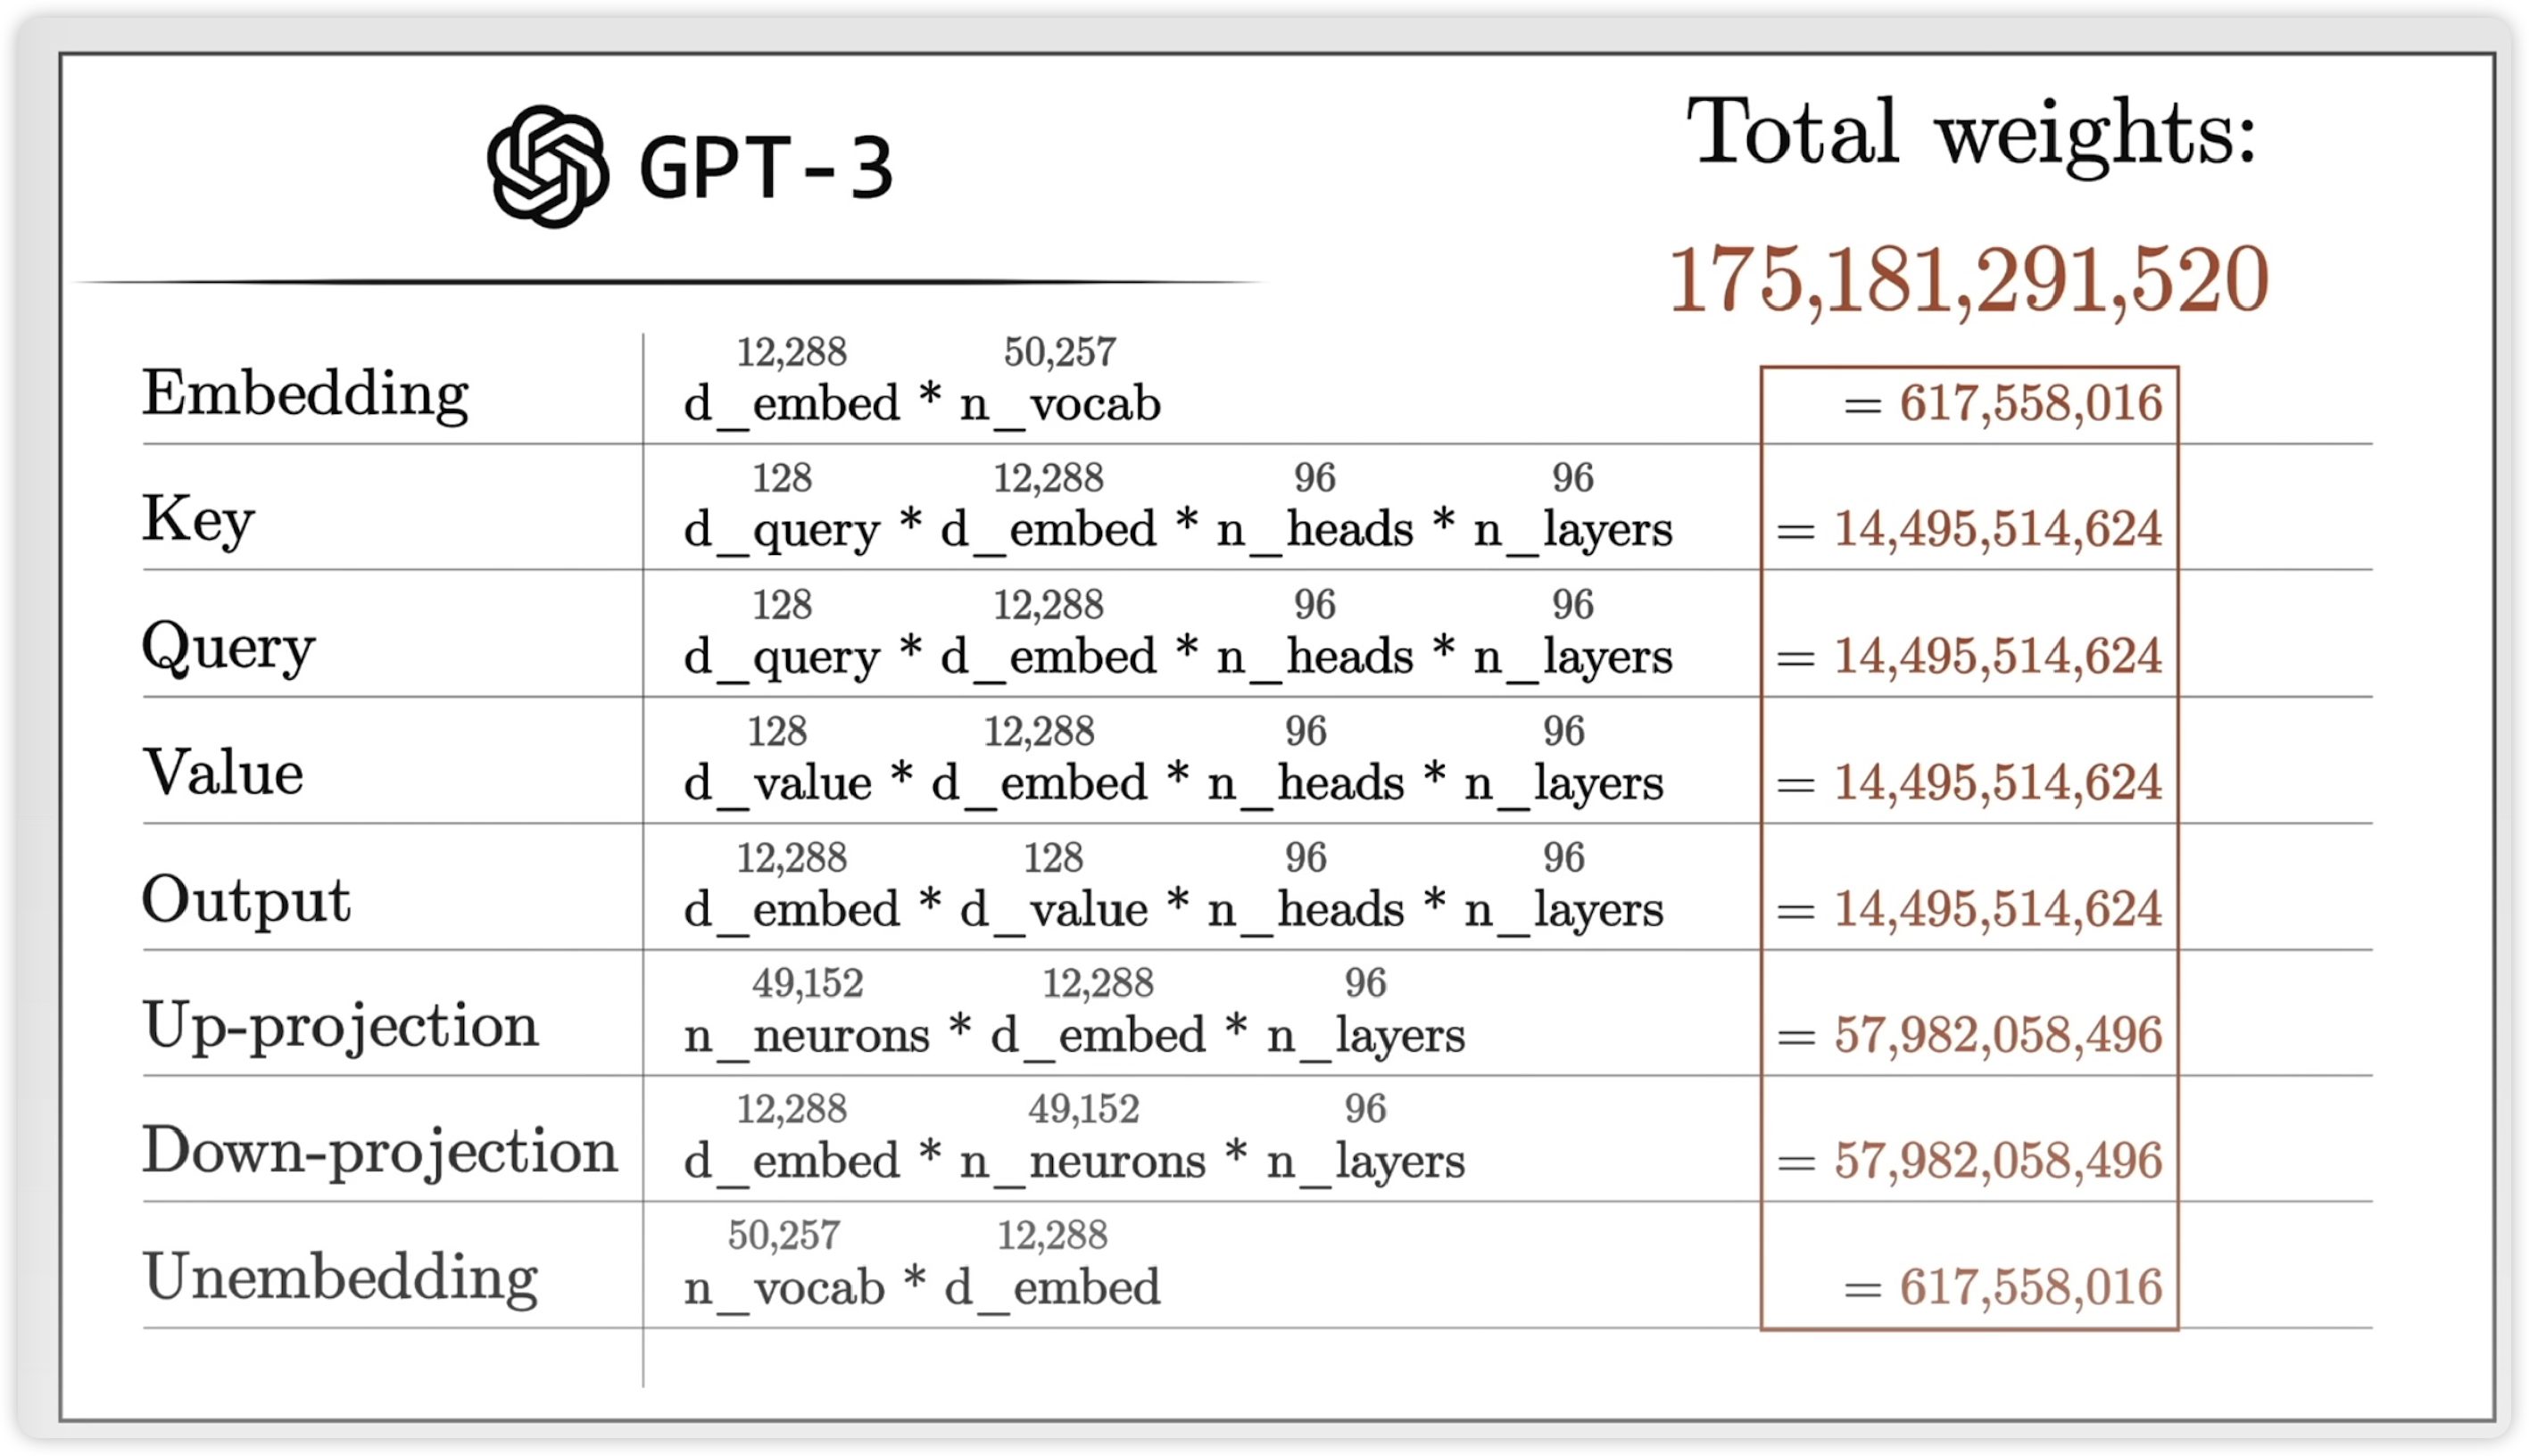
\includegraphics[width=0.8\textwidth]{figures/GPT3.png}
		\caption{Understanding the GPT-3 Architecture and Weight Distribution}
	\end{figure}

	\begin{figure}
		\centering
		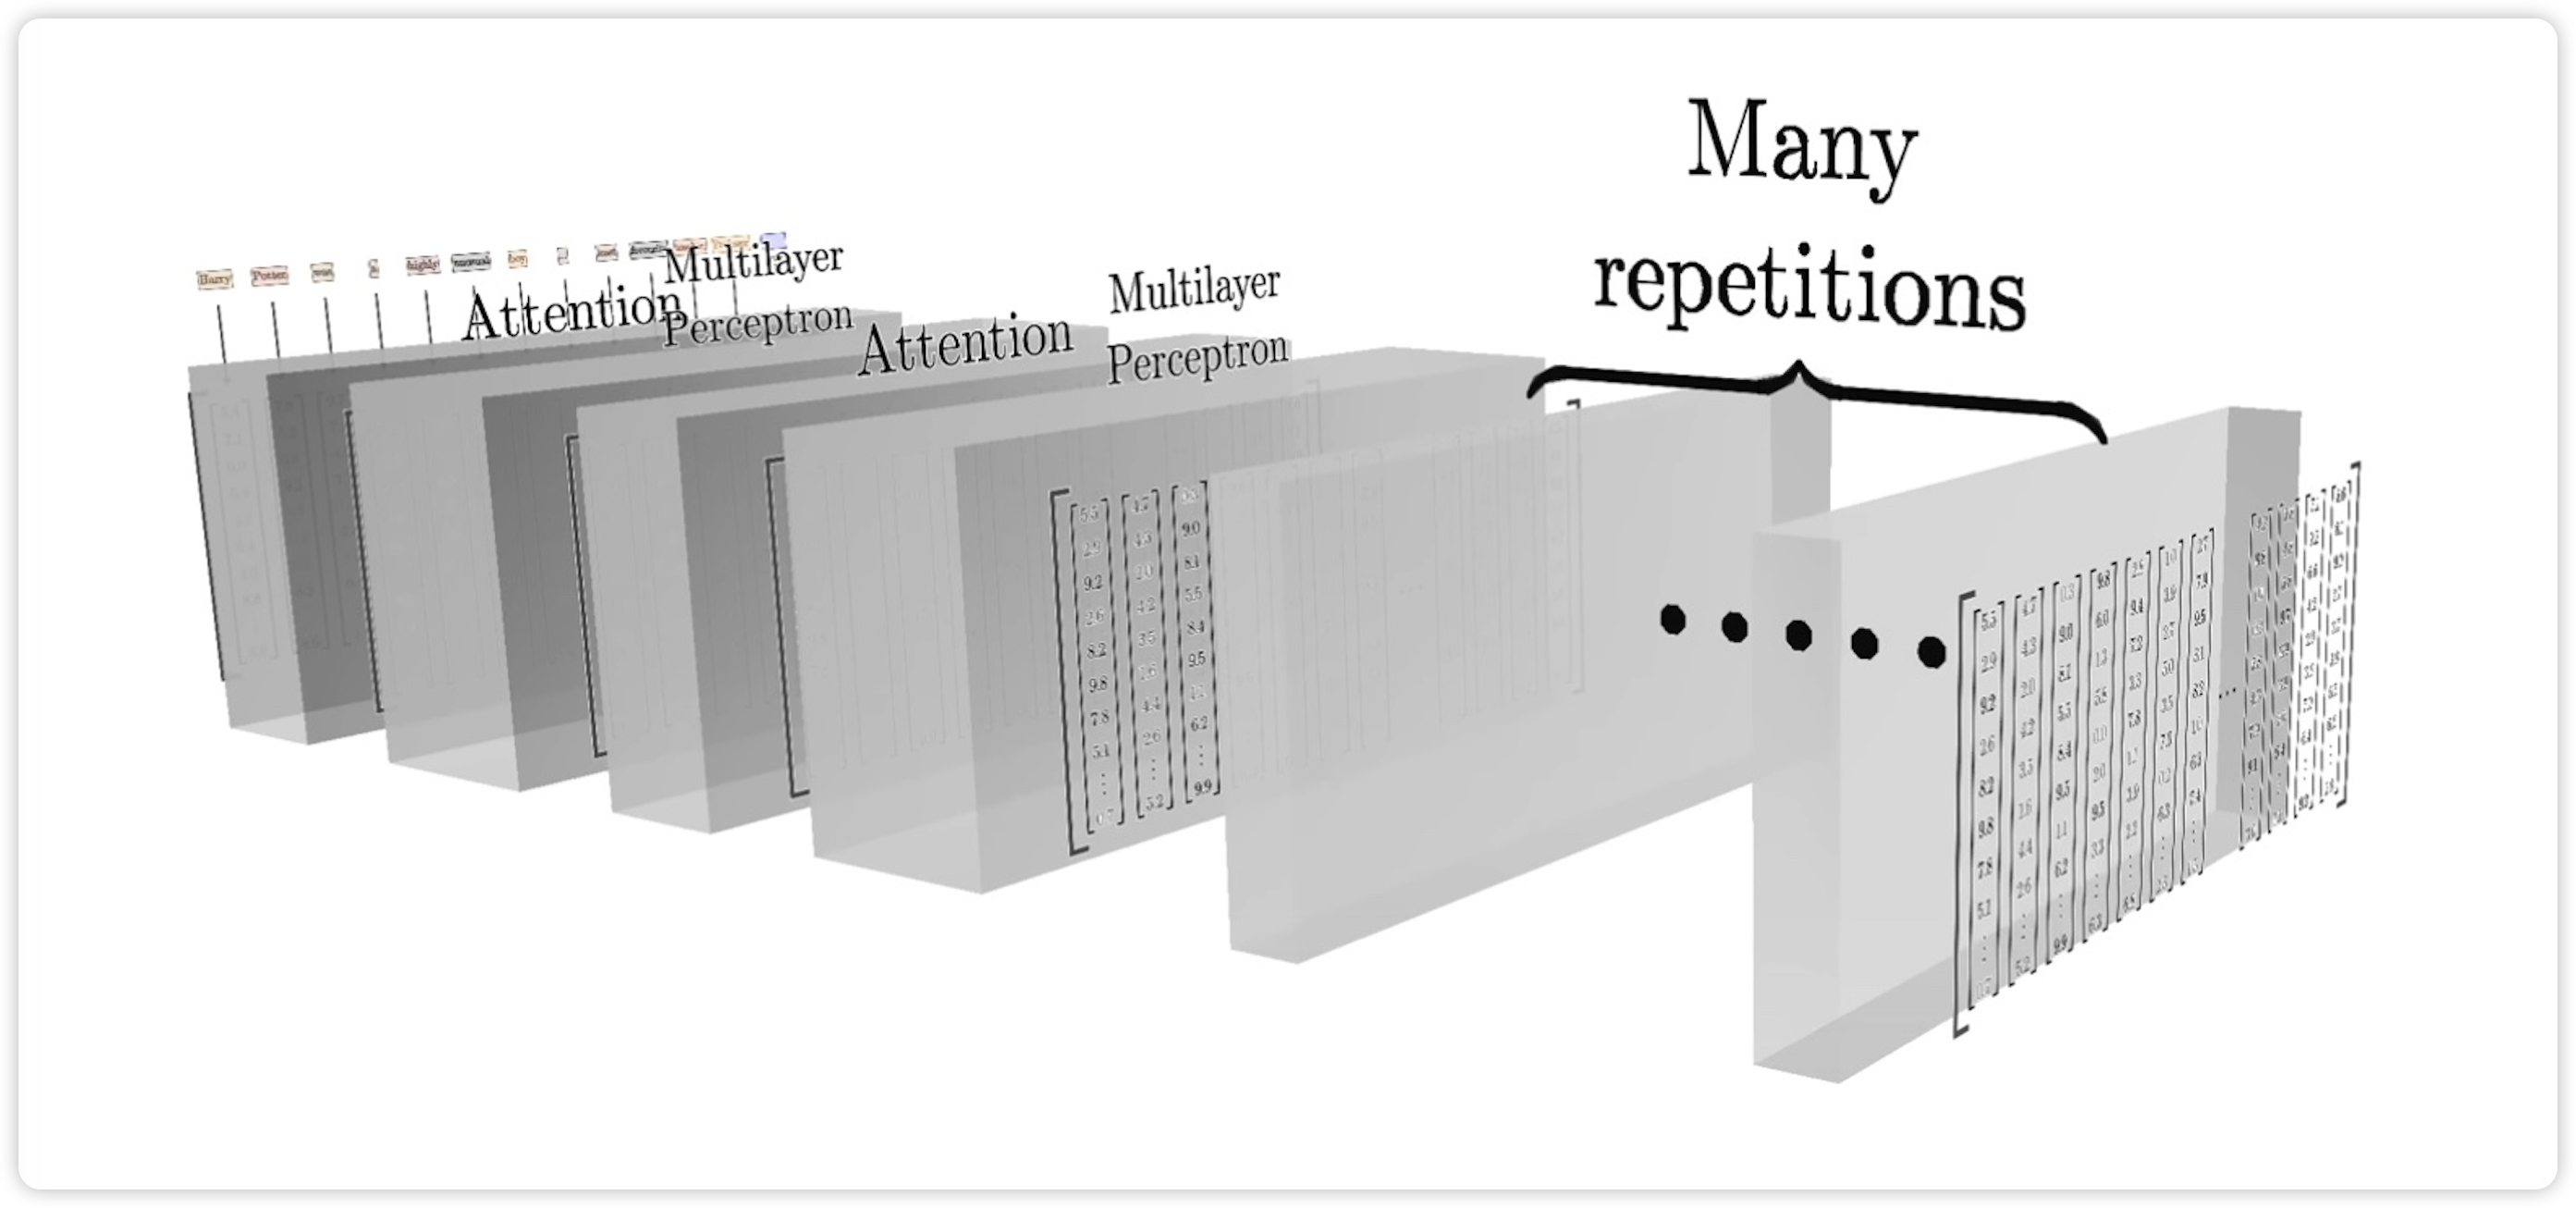
\includegraphics[width=0.8\textwidth]{figures/ModalNet-30.png}
		\caption{Model architecture of GPT-3}
	\end{figure}

	GPT-3's transformer architecture, rich with 175 billion parameters, harnesses parallel processing and attention mechanisms for advanced pattern recognition and language understanding. This structure facilitates coherent, context-aware text generation, surpassing prior models in complex language tasks.

    \end{block}
	\begin{block}{The Transformer}
	\textbf{Model Architecture}

	This figure provides a schematic representation of the Transformer model, illustrating its innovative encoder-decoder structure. The key components are as follows:
	\begin{itemize}
		\item \textbf{Encoder}: The Transformer model consists of N stacked layers, with each hosting a multi-head self-attention mechanism and a feed-forward network. Residual connections and layer normalization are applied around these sub-layers for efficiency.
	\end{itemize}
	\end{block}
    \end{column}

    \begin{column}{.3\linewidth}
      \begin{ntblock}
		\begin{figure}
			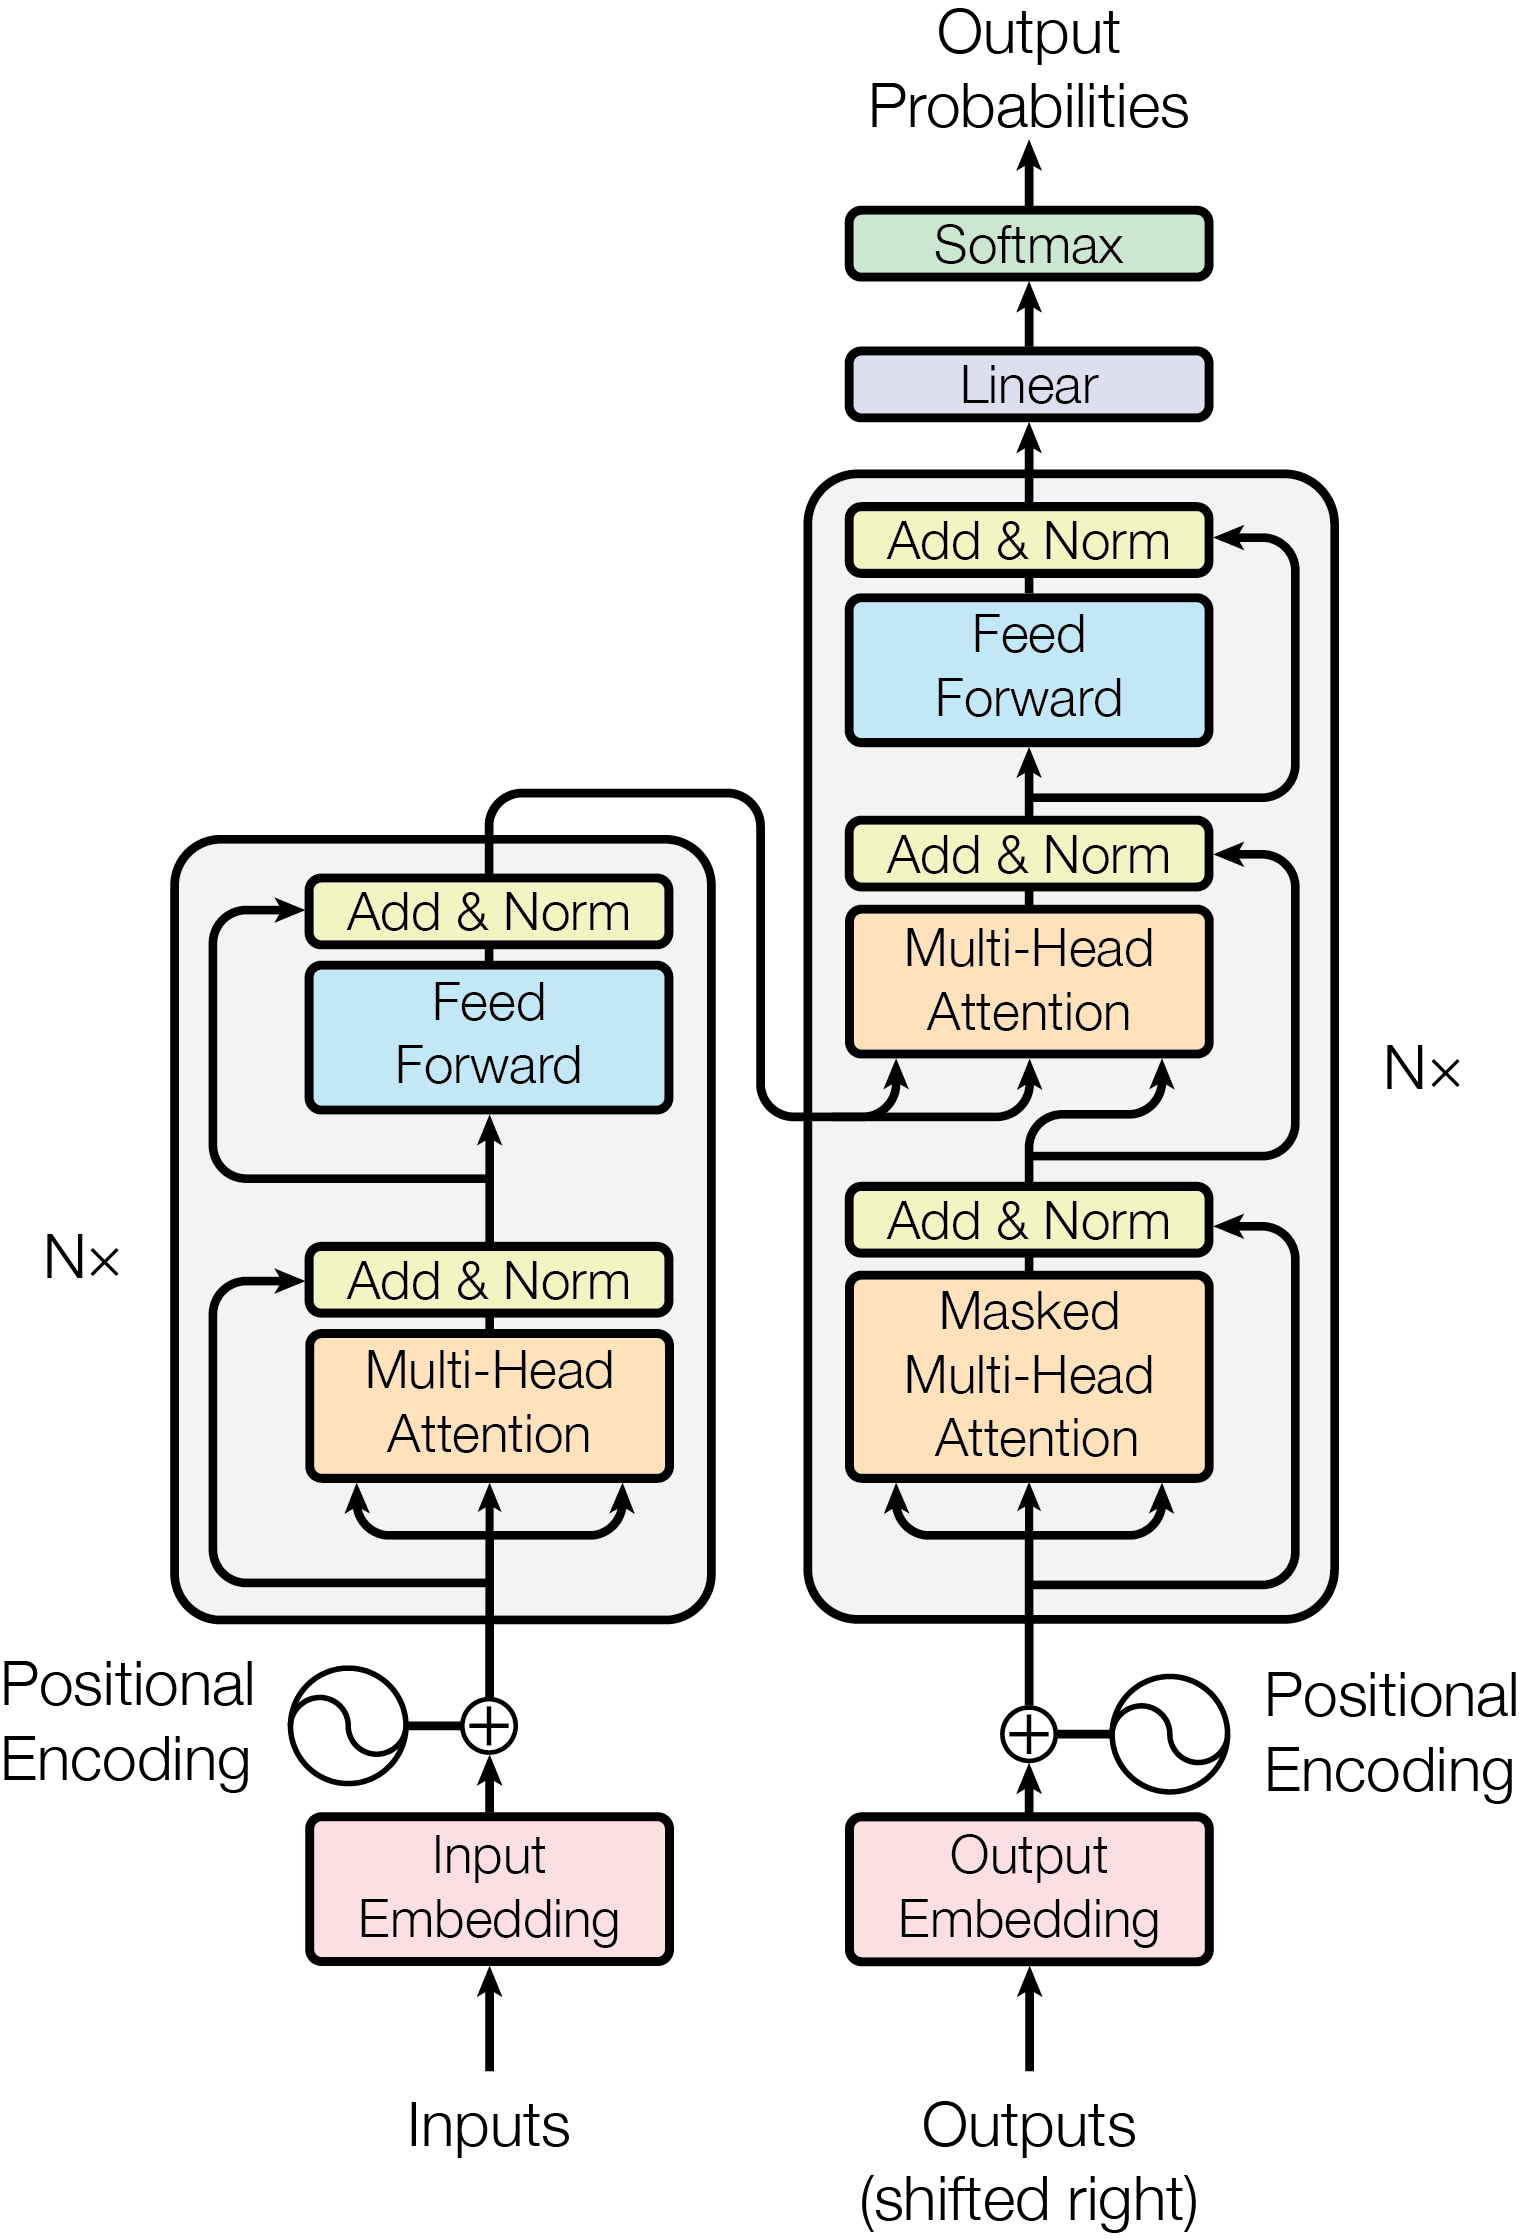
\includegraphics[width=0.8\textwidth]{figures/ModalNet-21.png}
			\caption{The Transformer - model architecture}
		\end{figure}
		\begin{itemize}
			\item \textbf{Decoder}: Also consists of N identical layers, with an additional third sub-layer in each that performs multi-head attention over the encoder's output. Similar to the encoder, the decoder employs residual connections and layer normalization.
		\end{itemize}

	\vspace{1em}
	\textbf{Attention Mechanism}

	This figure is divided into two main parts, illustrating the core mechanisms that enable the Transformer's powerful performance:
	\begin{itemize}
	\item \textbf{Scaled Dot-Product Attention (Left)}: Demonstrates the mechanism where the attention score is computed by scaling the dot product of queries and keys. This scaling factor, the inverse square root of the key dimension, helps in stabilizing the gradients. The attention scores determine how much each value is expressed at a position, facilitating focused processing of the input.
	\item \textbf{Multi-Head Attention (Right)}: Showcases how the Transformer extends the single attention process to multiple heads, allowing the model to jointly attend to information from different representation
	\end{itemize}
	\end{ntblock}
    \end{column}

    \begin{column}{.3\linewidth}
	\begin{ntblock}
	\begin{figure}
		\centering
		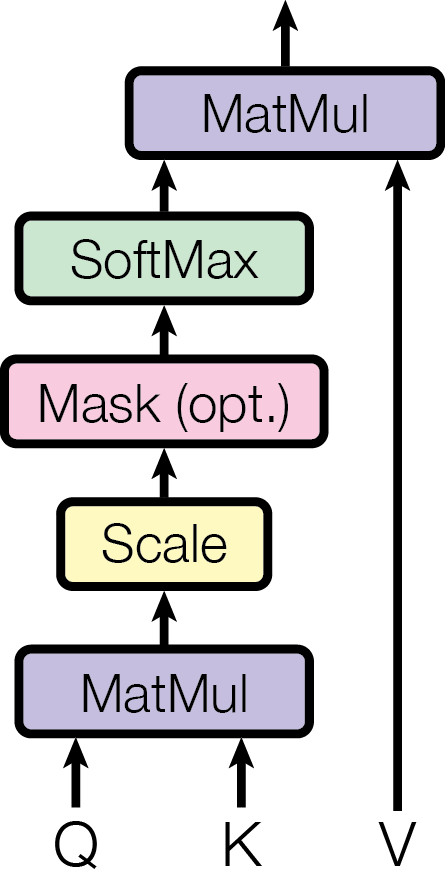
\includegraphics[width=0.33\textwidth]{figures/ModalNet-19.png}
		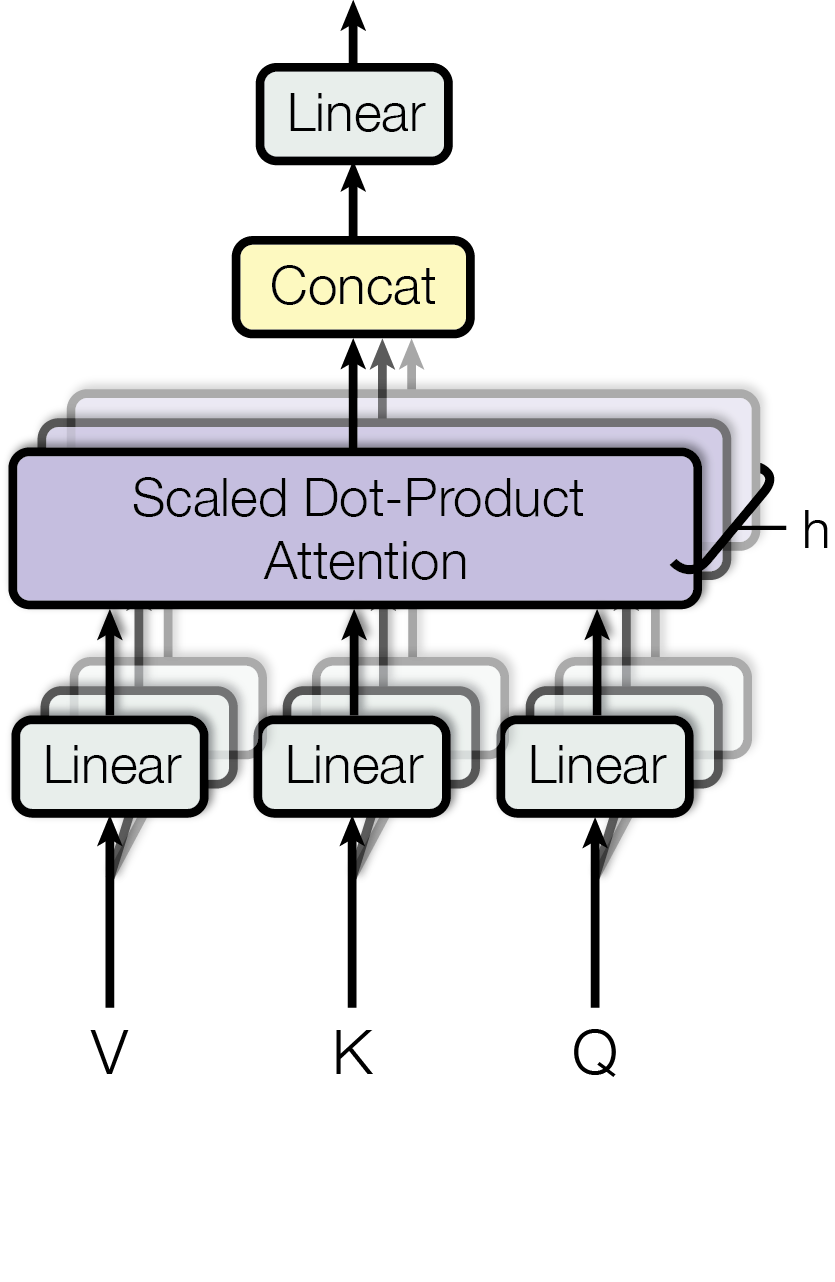
\includegraphics[width=0.33\textwidth]{figures/ModalNet-20.png}
		\caption{Attention Mechanisms in the Transformer}
	\end{figure}
	\begin{itemize}
		\item[]  subspaces at different positions. By projecting the queries, keys, and values multiple times with different learned linear projections, enhances the model's ability to capture varied dependencies. 
	\end{itemize}
	\end{ntblock}

	\begin{block}{Intelligence VS Human}
	\begin{figure}
		\centering
		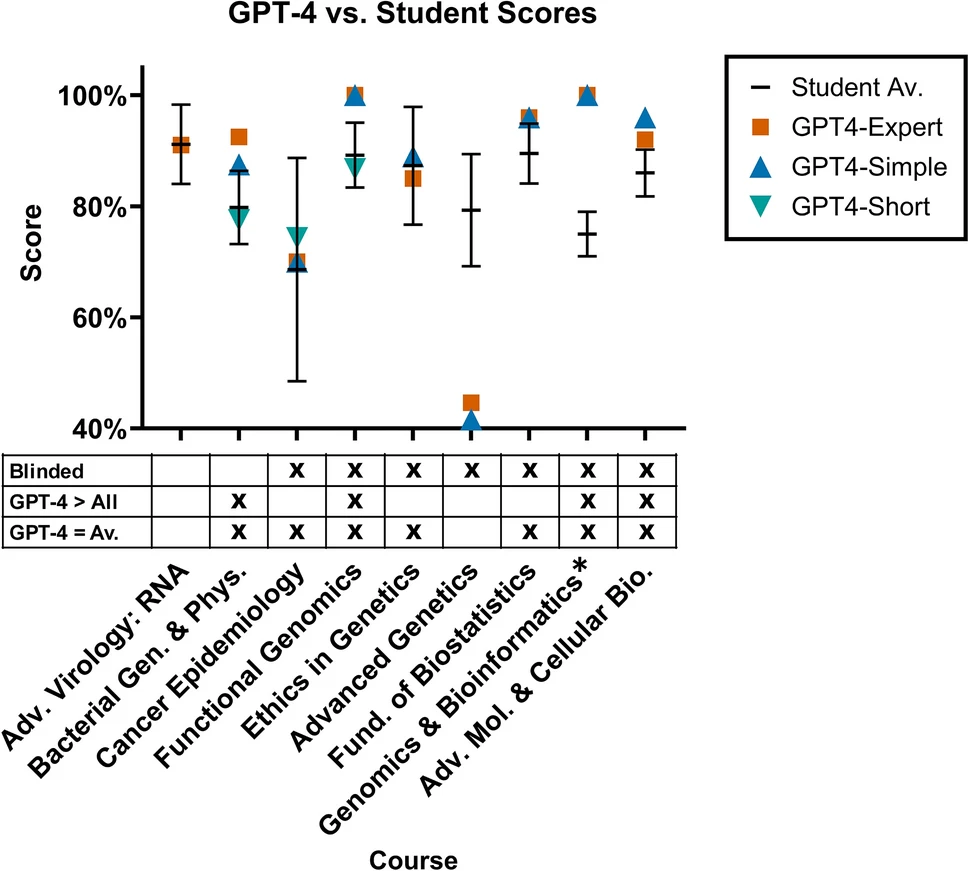
\includegraphics[width=0.55\textwidth]{figures/GPTvsHuman.png}
		\caption{GPT Performance On 9 Graduate Examinations.}
	\end{figure}
	Table Legend—Blinded: All GPT-4 exam grading was performed blinded in parallel with student assessments; GPT-4$>$All: One or more GPT-4 scores exceeded all student scores; GPT-4$\geq$Av.: One or more GPT-4 scores exceeded the average student score. 

	\end{block}
	\begin{block}{Acknowledgements}
		We are grateful to Nal Kalchbrenner and Stephan Gouws for
		their fruitful comments, corrections and inspiration.
	\end{block}

    \end{column}
  \end{columns}
\end{frame}

\end{document}
